\documentclass{beamer}
\usepackage[utf8]{inputenc}
\usepackage{hyperref}
\usepackage{multicol}
\usepackage{hyperref}
\usepackage{amsmath}
\usepackage[english]{babel}
\usepackage{algorithm}
\usepackage[noend]{algpseudocode}

\inputencoding{utf8}

\mode<presentation> {
    \usetheme{Madrid}
}

\usepackage{graphicx}
\usepackage{booktabs}

\title[Tiempo Lineal]{Ordenamiento en tiempo lineal}
\author{Ernesto Rodriguez - Juan Roberto Alvaro Saravia}
\institute{
    Universidad Francisco Marroquin \\
    \medskip \textit{ernestorodriguez@ufm.edu - juanalvarado@ufm.edu}
}

\date[\today]{}

\begin{document}

\begin{frame}
\titlepage
\end{frame}

\begin{frame}
\frametitle{Ordenamiento por conteo}
\begin{itemize}
    \item{Los elementos que se desean ordenar son enteros}
    \item{Todo elemento siendo ordenado es menor o igual que alg\'un $k$}
    \item{Cuando $k\cong n$, entonces la complejidad es $\mathcal{O}(n)$}
    \item{Consiste en contar la cantidad de valores menores a cada uno
    de los valores en el arreglo de entrada.}
    \item{Luego de contar los valores, cada valor se puede colocar
    en su posici\'on correspondiente.}
\end{itemize}
\end{frame}

\begin{frame}
    \frametitle{Ordenamiento por conteo}
    \begin{algorithm}[H]
        \caption{Ordenamiento por conteo}
        \begin{algorithmic}[1]
        \Procedure{OrdenarConteo}{$As$,$Bs$,$k$}
        \State{{\bf let} $Cs[k]$}
        \For{$i\gets 1$ {\bf to} $k$}
        \State{$Cs[i]\gets 0$}
        \EndFor
        \For{$i\gets 1$ {\bf to} $\mathtt{len}(As)$}
        \State{$Cs[As[i]]\gets Cs[As[i]] + 1$}
        \EndFor
        \For{$i\gets 2$ {\bf to} $k$}
        \State{$Cs[i]=Cs[i]+Cs[i-1]$}
        \EndFor
        \For{$i\gets \mathtt{len}(As)$ {\bf downto} $1$}
        \State{$Bs[Cs[As[i]]]\gets As[i]$}
        \State{$Cs[As[i]]\gets Cs[As[i]]-1$}
        \EndFor
        \EndProcedure
        \end{algorithmic}
    \end{algorithm}
\end{frame}

\begin{frame}
    \frametitle{Ordenamiento por conteo}
    \begin{itemize}
        \item{Logra mejor rendimiento que los algoritmos de comparaci\'on
        cuando $k\cong n$}
        \item{El algoritmo nunca compara los valores que esta ordenando}
        \item{El algoritmo utiliza el valor numerico absoluto de cada
        elemento para obtener su posici\'on final.}
        \item{Requiere memoria en el odren de $\mathcal{O}(k)$}
    \end{itemize}
\end{frame}

\begin{frame}
    \frametitle{Radix sort}
    \begin{itemize}
        \item{Dado un numero, se utiliza su representaci\'on decimal
        (u octal, binaria, hexadecimal, ect.)}
        \item{Se ordenan los valores mediante varias ``pasadas''}
        \item{En cada ``pasada'', se escoge uno de los digitos de los
        valores siendo ordenado como indice de ordenamiento.}
        \item{El algoritmo procede ordenanto primero el digito menos
        significativo hasta llegar al digito m\'as significativo.}
        \item{El algoritmo procede hasta haber ordenado respecto
        a todos los digitos.}
    \end{itemize}
\end{frame}

\begin{frame}
    \frametitle{Radix Sort}
    \begin{center}
    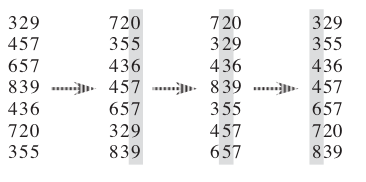
\includegraphics[width=8cm]{./radix.png}
    \end{center}
\end{frame}

\begin{frame}
    \frametitle{Radix sort}
    \begin{algorithm}[H]
        \caption{Radix sort}
        \begin{algorithmic}[1]
        \Procedure{RadixSort}{$As$,$d$}
        \For{$i\gets 1$ {\bf to} d}
            \State{Utilizar un algoritmo de ordenamiento estable}
            \State{para ordenar respecto al digito i}
        \EndFor
        \EndProcedure
        \end{algorithmic}
    \end{algorithm}
\end{frame}

\end{document}